\newpage

\section{WS Clock} 

\subsection{Теория по алгоритму.}
Прежде чем перейти к алгоритму WS Clock, нужно обговорить и определить некоторые моменты и определения, встречающиеся в описании данного алгоритма.\\
Начнём с краткого описания определений, входящих в понятия "рабочий набор". \\
Замещение страниц по запросу - это когда страницы загружаются только по требованию, а не заранее, то есть наш процесс прерывается и ждет полной загрузки страницы. \\ 
Буксование - это когда каждую последующую нужную нам страницу приходится процессу загружать в память.\\
Для того чтобы не происходило частых прерываний, желательно чтобы часто использовавшиеся страницы загружались заранее, а остальные подгружались уже по необходимости.\\
Рабочий набор - это множество страниц (к), которое процесс использовал до некоторого момента времени (t).

\begin{figure}[h]
\center{\includegraphics[width=1\linewidth]{gr.gif}}
\caption{Зависимость рабочего набора w(k,t) от количества запрошенных страниц.}
\end{figure}

Другими словами рабочий набор переходит в насыщение, значение w(k,t) в состояние насыщения может служить для рабочего набора, который необходимо загружать именно до запуска процесса, не иначе\\
Теперь переходим к нашему алгоритму. WS Clock является модификацией алгоритма "рабочий набор". Для его использования необходима структура данных, которая представляет собой кольцевой список. В начальном положении этот список пуст. Когда же мы загружаем первую страницу, она добавляется в список и занимает положение "во главе". По мере "прихода" страниц они поступают в список, формируя замкнутое кольцо. Каждая запись, кроме бита R и бита M, содержит поле под названием «время последнего использования» из базового и уже выше упомянутого  алгоритма «рабочий набор».\\
Так же, как и в случае алгоритма «часы», при каждом, буквально каждом страничном прерывании первой будет проверятся та страница, на которую указывает стрелка наших "часов". Если бит R=1, то это значит, что страница использовалась в течение последнего такта времени, из-за она не является нашим претендентом на удаление. Тогда бит R устанавливается на 0, а стрелка двигается к следующей странице и для нее повторяется наш алгоритм.\\ 
Если же в момент проверки бит R=0 и время последнего использования больше "возраста страницы" T, то начинаем проверять бит M – были ли внесены изменения в нём. Если нет, то страница является нашей целью на удаление. Если изменения были – страница помечается как необходимый кандидат для копирования, а стрелка "часов" сдвигается.\\ 

\begin{figure}[h]
\center{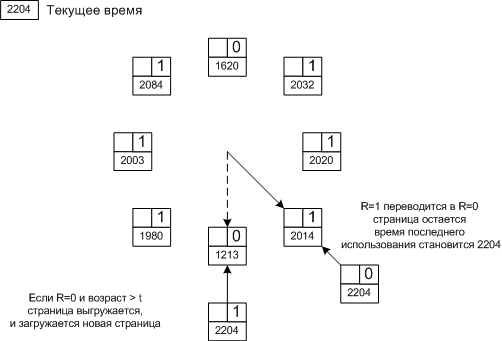
\includegraphics[width=1\linewidth]{al.PNG}}
\caption{Работа алгоритма WSClock.}
\end{figure}

Если стрелка обходит полный круг и возвращается обратно, то возможно всего два варианта: \\
1) существует запланированная операция переноса страницы на диск; \\
2) вообще ничего не запланировано. \\
В первом варианте будет выбрана первая попавшаяся страница без изменений с битом R=0. Во втором случае нам предъявляются права на совершенно любую страницу. \\
Одним из наилучших алгоритмов является как раз алгоритм WSCIock. Он обеспечивает хорошую постраничную подкачку.\\ 
Но как и у любого алгоритма у него есть тоже недостатки – размеры страниц и частота страничных прерываний достаточно сильно влияют на производительность нашего алгоритма, все данные находятся в состояние "хаоса", то есть они перемешаны друг с другом. 

\section{Работа алгоритма WSClock.}
full – количество заполненных ячеек в памяти;
time – время таймера;
timeClear – время чистого замещения; 
timeDirty – время грязного замещения;
RamSize – размер оперативной памяти
CCount – счётчик чистых страниц; 
DCount – счётчик грязных страниц;
[ ]R – массив R; 
[ ]M – массив бита M;
pointer - указатель на страницу;
numberOfAppeal - номер обращения;
[ ] numbersOfAppeal - массив для запоминания номера обращений (для каждой ячейки памяти запоминаем когда к странице из этой ячейки последний раз обращались)
T - количество обращений, через которые страница не будет относится к рабочему набору
calls – количество обращений к странице;
numbers – размер виртуальной памяти;
Page – номер страницы к которой идёт обращение;
[ ]frame – массив для номеров страниц, которые уже в оперативной памяти;
planned – массив на запись;
temp – страницы, которые будет заменять;
n – максимальное количество страниц;
notChangedPage – указатель, который показывает на страницу во время прерывания;
repptr – указатель на заменяемую страницу;
pointer – указатель;
begin – начальное положение стрелки;
WrittentoDisk – запись на диск;

Количество мест в памяти, как известно, ограничено. Когда все места заполнены, но нам нужно добавить новую страницу, происходит прерывание. И вот вследствие этого прерывания начинает работать алгоритм замещения страниц.  Когда же места хватает, алгоритм замещения страниц нам не нужен, следовательно, он не начинает свою работу. Просто происходит добавление страницы в память и увелечение счётчика чистых замещений.\\
Изначально стрелка “часов” располагается в начале, но прерывание может застать нашу стрелку не в начале её пути. Для такого случая мы используем notChangedPage. notChangedPage задаёт нам начальную страницу проверки. Для начала в алгоритме мы проверяем бит М. Он равен нулю, а бит R равен одному, то мы продолжаем искать страницу для удаления. Данную станицу причесляем к чистой, следовательно увеличиваем счётчик чистых страниц. Указатель смещаем вперед. Теперь начнём с бита R. Вот мы нашли бит R равный нулю, проверяем бит М, если он равен одному, то мы помечаем страницу, как необходимую для записи. Дальше мы увеличиваем счётчик planned и записываем страницу на диск. В это случае  repptr становится pointer и так же происходит увеличение счётчика грязных страниц.  В случае, когда бит M равен нулю происходит удаление странице и это место занимает наша новая страница.

\subsection{Код алгоритма.}







